\clearpage
\section{$\beta$-Funktion im $\mathbb{R}^2$}\label{beta_im_R2}
   Um 2-dimensionale autonome DGL-Systeme zu veranschaulichen eignet sich das 
   Bild des Kopplungskonstanten-Flusses. Dabei "`fließt"' ein Anfangswert 
   $\alpha(t_0)$ mit Geschwindigkeit und Richtung $\dot\alpha(t) = 
   \beta(\alpha(t))$ entlang einer Trajektorie durch 
   den Phasenraum. Der Satz von Picard-Lindelöf stellt dabei sicher, dass 
   sich zwei Trajektorien nicht schneiden. Ein Flussdiagramm wie in Abbildung 
   \ref{beta_allgemein:fig:fluss_beispiel} zeigt das Verhalten von $\alpha(t)$ 
   indem das Geschwindigkeitsfeld $\beta$ durch Pfeile im Phasenraum 
   dargestellt wird.
      \begin{figure}[h]
    \centering
    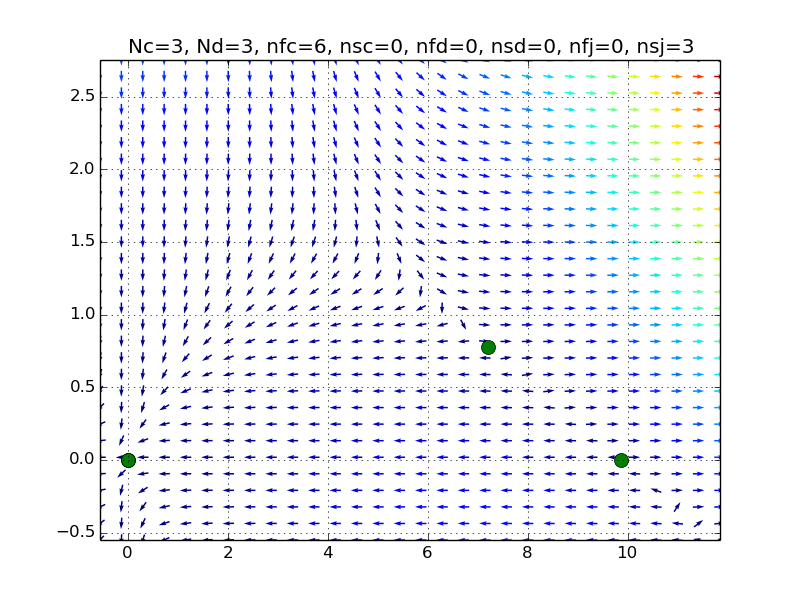
\includegraphics[scale=0.5]{abschnitte/beta_im_R2/fig/flow_example.png}
    \caption{Ein Flussdiagramm für $\beta(\alpha_1,\alpha_2 )$.}
    \label{beta_allgemein:fig:fluss_beispiel}
   \end{figure}


  \subsection{Stabilitätsbedingungen}
    Für ein System mit zwei Kopplungskonstanten vereinfacht sich die 
    Untersuchung erheblich, da der Phasenraum der $\mathbb{R}^2$ ist und, wie in 
    Abschnitt \ref{Schleifen} gezeigt wurde, die Stabilitätsmatrix allgemein 
    die Form
	\begin{equation}
	 \dbda = \begin{pmatrix}
	          \sum\limits_{i=2,j=0}i \alpha_1^{i-1} \alpha_2^j X^1_{ij} &
	          \sum\limits_{i=2,j=1}j \alpha_1^i \alpha_2^{j-1} X^1_{ij}\\
	          \sum\limits_{i=1,j=2}i \alpha_1^{i-1} \alpha_2^j X^2_{ij} &
	          \sum\limits_{i=0,j=2}j \alpha_1^i \alpha_2^{j-1} X^2_{ij}
	         \end{pmatrix}\label{eq:beta_im_R2:stab_matrix}
	\end{equation}
    annimmt. Die Eigenwerte von $\dbda$ können explizit 
    als\begin{equation}
    \lambda_{+/-}=\frac12 \Sp \pm \sqrt{ \left( \frac{\Sp}{2} \right)^2-\Det } 
    \label{eq:beta_im_R2:lambda}
    \end{equation}
    angegeben werden. Es wird nun kurz begründet, warum ein vollständig 
    wechselwirkender Fixpunkt im allgemeinen als hyperbolisch angenommen 
    werden darf, danach wird gezeigt, dass teilweise wechselwirkende Fixpunkte 
    für beliebig hohe Ordnung nicht-hyperbolisch sind. Im $2$-dimensionalen 
    lässt sich jedoch ein alternatives Stabilitätskriterium für solche 
    Fixpunkte finden.
    \subsubsection{hyperbolischer Fixpunkt}
      Sind $\Sp$ und $\Det$ nicht Null, lässt sich das Vorzeichen der 
      Eigenwerte leicht Nachrechnen, das Ergebnis ist in Tabelle 
      \ref{beta_im_R2:tab:stabilitaet_hyperbolisch} zu sehen.
  
      \begin{table}[h]
	\centering
	\begin{tabular}{ccccc}
	\toprule \midrule
	 $\Sp $& $\Det $ & $\Re\lambda_+$ &$\Re\lambda_-$ & UV-Verhalten \\
	 \midrule 
	 $>0$	& $>0$	&$>0$ & $>0$	& repulsiv   \\
	 $<0$	& $>0$	&$<0$ & $<0$	& attraktiv  \\
	  -     & $<0$	&$>0$ & $<0$	& Sattelpunkt\\
	  \midrule
	  \bottomrule
	\end{tabular}
	\caption{Das UV-Verhalten hyperbolischer Fixpunkte für $\Sp\neq0$ 
	und $\Det \neq 0$.}
	\label{beta_im_R2:tab:stabilitaet_hyperbolisch}
\end{table}
      
      Da man in der Reihenentwicklung der $\beta$-Funktion davon ausgeht, 
      dass höhere Ordnungen vernachlässigbar klein werden, kann man davon 
      ausgehen, dass hyperbolische Fixpunkte der 
      Ordnung $n$ auch für höhere Ordnungen hyperbolisch bleiben. Falls ein 
      vollständig wechselwirkender Fixpunkt $(\alpha_1^*\neq 0,
      \alpha_2^*\neq 0)$ in Ordnung $n$ entweder $\left.\Sp \right|_*=0$ 
      oder $\left. \Det \right|_*=0$ ergibt, kann man davon ausgehen, dass 
      sich die Koeffizienten $X^k_{ij}$ zufällig aufheben und der Fixpunkt in 
      höherer Ordnung wieder hyperbolisch wird. Vollständig 
      wechselwirkende nicht-hyperbolische Fixpunkte können also als Folge 
      einer zu groben Berechnung der $\beta$-Funktion verstanden werden. 
      Es ist nicht klar, ob der Eigenvektor $e_i$ zum Eigenwert $\lambda_i=0$ 
      eine UV-attraktiven oder repulsiven Richtung entspricht, da sich dies 
      jedoch direkt auf die Dimension der kritischen Hyperfläche auswirkt ist 
      die Untersuchung solcher Fixpunkte nur bedingt sinnvoll.

    \subsubsection{nicht-hyperbolischer Fixpunkt}\label{beta_im_R2:nicht-hyperbolischer_Fixpunkt}
%       In dem Fall, dass bei $\alpha^*$ ein Eigenwert 
%       verschwindet, ist $\left.\Det\right|_*=\lambda_+|_* \lambda_-|_* = 0$ und
%       \begin{alignat}{3}
%       &\left.\lambda_+\right|_* = \left.\Sp\right|_* \quad && \lambda_-|_*=0  
%       \quad && \text{für }\left.\Sp\right|_*\geq 0 \\
%       &\lambda_+|_* = 0   \quad && \lambda_-|_*=\left.\Sp\right|_*  \quad && 
%       \text{für }\left.\Sp\right|_*\leq 0 
%       \quad .
%       \end{alignat}
%       Außerdem 
%       \begin{equation}
% 	\left.\frac{\partial \lambda_{+/-}}{\partial \alpha_i}\right|_*=
% 	\left[-\frac{1}{2} \frac{\partial \Sp}{\partial \alpha_i} 
% 	+ \frac{1}{\lambda_{-/+} }
% 	\frac{\partial \Det}{\partial \alpha_i} \right]_*
% 	\quad ,
%       \end{equation}
%       wobei $\lambda_{+/-}|_*$ der verschwindende Eigenwert ist.
	 Ein teilweise wechselwirkender Fixpunkt, o.E. 
	 $\alpha^*=(\alpha_1^*,0)$,  
	 führt zu der Stabilitätsmatrix 
	 \begin{equation}
	 \dbdafix = \begin{pmatrix}
	          \sum\limits_{i=2}i (\alpha_1^*)^{i-1}  X^1_{i0} &
	          \sum\limits_{i=2} (\alpha_1^*)^i  X^1_{i1}\\
	          0&
	          0
	         \end{pmatrix} \quad . \label{eq:beta_im_R2:stab_matrix_0}
	 \end{equation}
	 mit den Eigenvektoren und Eigenwerten
	 \begin{equation}
	 e_1=\begin{pmatrix}1 \\0 \end{pmatrix} \quad , \quad
	 e_2\propto\begin{pmatrix}
		  -\sum_{i=2} (\alpha_1^*)^i X^1_{i1} 
		   \\
		  \sum_{i=2}i (\alpha_1^*)^{i-1}  X^1_{i0} 
	           \end{pmatrix} \quad , \quad
	 \lambda_1 = \sum_{i=2}i (\alpha_1^*)^{i-1}  X^1_{i0} \quad , \quad
	     \lambda_2=0      \quad .
	 \end{equation}
	Da in $\beta_2$ die Variable $\alpha_2$ in jedem Monom  
	 mindestens zur zweiten Potenz auftaucht, ist dies für 
	 beliebig hohe Ordnung zu erwarten, sodass hier ein alternatives Kriterium 
	 für das UV-Verhalten des Fixpunktes gefunden werden muss.  


	Zunächst wird \eqref{eq:beta_allgemein:beta_linear} um die zweite 
	Ordnung der Taylorentwicklung ergänzt,
     \begin{equation}
     \beta_i(\alpha) \simeq \sum\limits_{m=1}^2 \left. \frac{\partial \beta_i
     }{\partial
      \alpha_m}\right|_* \left(\alpha_m-\alpha^*_m\right) + \frac12 
      \sum\limits_{m,n=1}^2 
       \left(\alpha_m-\alpha^*_m\right)
      \left.\frac{\partial^2 \beta_i}{\partial\alpha_m \partial\alpha_n}
      \right|_* \left(\alpha_n-\alpha^*_n\right) \quad .
      \end{equation}
%      oder in vektorieller Schreibweise in der Basis der Eigenvektoren
%      \begin{equation}
%      \ddt (K_1e_1+K_2e_2)\simeq\dbdafix (K_1e_1+K_2e_2) +
%      (K_1e_1+K_2e_2) \cdot \left.\left(\nabla \dbda \right)\right|_*
%       (K_1e_1+K_2e_2) \quad .
%      \end{equation}
%     Es werden die Ableitungen der Stabilitätsmatrix benötigt
%     \begin{align}
%      \left.\frac{\partial}{\partial \alpha_1} \frac{\partial \beta_i}{\partial 
%      \alpha_n}\right|_* &= \left. 
%      \begin{pmatrix}
% 	\sum\limits_{i=2,j=0} i (i-1) \alpha_1^{i-2}\alpha_2^j X_{ij}^1 &
% 	\sum\limits_{i=2,j=1} ij \alpha_1^{i-1}\alpha_2^{j-1} X_{ij}^1 \\
% 	\sum\limits_{i=2,j=2}i(i-1) \alpha_1^{i-2} \alpha_2^j X_{ij}^2 &
% 	\sum\limits_{i=1,j=2} ij \alpha_1^{i-1}\alpha_2^{j-1} X_{ij}^2
%      \end{pmatrix}_{in} \right|_*   \\
%      &=\begin{pmatrix}
% 	\sum\limits_{i=2} i (i-1) \alpha_1^{i-2} X_{ij}^1 &
% 	\sum\limits_{i=2} i \alpha_1^{i-1} X_{i1}^1 \\
% 	0 &0
%      \end{pmatrix}_{in}
%     \end{align}
%     
%     \begin{align}
%      \left.\frac{\partial}{\partial \alpha_2} \frac{\partial \beta_i}{\partial 
%      \alpha_n}\right|_* &= \left. 
%      \begin{pmatrix}
% 	\sum\limits_{i=2,j=1} i j \alpha_1^{i-1}\alpha_2^{j-1} X_{ij}^1 &
% 	\sum\limits_{i=2,j=2} j(j-1) \alpha_1^{i}\alpha_2^{j-2} X_{ij}^1 \\
% 	\sum\limits_{i=1,j=2}ij \alpha_1^{i-1} \alpha_2^{j-1} X_{ij}^2 &
% 	\sum\limits_{i=1,j=2} j(j-1) \alpha_1^{i}\alpha_2^{j-2} X_{ij}^2
%      \end{pmatrix}_{in} \right|_*   \\
%      &=\begin{pmatrix}
% 	\sum\limits_{i=2} i  \alpha_1^{i-1} X_{i1}^1 &
% 	\sum\limits_{i=2} 2 \alpha_1^{i-1} X_{i2}^1 \\
% 	0 & 
% 	\sum\limits_{i=1} 2 \alpha_1^i X_{i2}^2
%      \end{pmatrix}_{in}
%     \end{align}
    Wie in Abschnitt \ref{beta_allgemein:Verhalten} wird diese Gleichung in 
    der Eigenbasis der Stabilitätsmatrix geschrieben
    \begin{align}
     \dot{K}_1 (t) e_1^i +\dot{K}_2 e_2^i &= \sum\limits_{k,m=1}^2
     K_k(t) \frac{\partial \beta _i}{\partial \alpha_m} e_k^m 
     + \frac12 \sum\limits_{k,l,m,n=1}^2
     K_k(t)K_l(t)\frac{\partial^2 \beta _i}{\partial \alpha_m \alpha_n}e_k^m  
     e_l^n \\
     &= K_1(t)\lambda_1 e_1^i  + \frac12 \sum\limits_{k,l,m,n=1}^2
     K_k(t)K_l(t)\frac{\partial^2 \beta _i}{\partial \alpha_m \alpha_n}e_k^m  
     e_l^n 
     \quad . \label{eq:beta_im_R2:zweite_ordnung}
    \end{align}
    Die Indizes $k$ und $l$ laufen dabei für die zwei Eigenvektoren, während 
    $m$, $n$ und $i$ für die Komponente eines Vektors stehen. Der 
    Koeffizientenvergleich in $e_1$ führt in erster Ordnung zum gleichen 
    Ergebnis wie beim hyperbolischen Fixpunkt. Auf der kritischen Hyperläche 
    gilt demnach $\lambda_1<0 \Rightarrow K_1(t)\rightarrow 0$ für $t$ groß, 
    oder $\lambda>0 \Rightarrow K_1(t)\equiv 0$, da der Fixpunkt sonst nicht 
    erreicht wird. Für große $t$ wird \eqref{eq:beta_im_R2:zweite_ordnung} 
    damit zu 
    \begin{align}
     \dot{K}_2 e_2^i &= \frac{1}{2} K_2(t)^2 \sum\limits_{m,n=1}^2 
     \frac{\partial^2 \beta_i}{\partial \alpha_m \partial \alpha_n} e_2^m e_2^n
     \\&= \frac12 K_2(t)^2 \sum\limits_{m,n=1}^2 \left[ \left(e_2^m 
     \frac{\partial}{\partial \alpha_m} \right) 
     \left(e_2^n \frac{\partial}{\partial \alpha_n} \right) - e_2^m 
     \frac{\partial e_2^n}{\partial \alpha_m} \frac{\partial}{\partial \alpha_m}
     \right]_* \beta_i \\
     &= \frac12 K_2(t)^2 \left[ \sum\limits_{m=1}^2 e_2^m 
     \frac{\partial\lambda_2}{\partial \alpha_m}e_2^i - \sum\limits_{m,n=1}^2 
     e_2^m \frac{\partial e_2^n}{\partial \alpha_m} 
     \frac{\partial}{\partial \alpha_n} \beta_i \right]_* \quad . 
     \label{eq:beta_im_R2:mischterm}
    \end{align}
    Für $i=2$ kann eine Lösung wie folgt gefunden werden. Der zweite Term in 
    \eqref{eq:beta_im_R2:mischterm} ist wegen 
    \eqref{eq:beta_im_R2:stab_matrix_0} gleich Null.
    Aus \eqref{eq:beta_im_R2:lambda} und \eqref{eq:beta_im_R2:stab_matrix} 
    erhält man am Fixpunkt
    \begin{equation}
     \frac{\partial \lambda_2}{\partial \alpha_q} = 
     \frac{\partial}{\partial \alpha_q} 
     \frac{\partial \beta_2}{\partial \alpha_2} -
     \frac{\partial \beta_1}{\partial \alpha_2} 
     \left(\frac{\partial \beta_2}{\partial \alpha_1} \right)^{-1}
     \frac{\partial}{\partial \alpha_q} 
     \frac{\partial \beta_2}{\partial \alpha_1} \quad 
         \begin{cases}
     =0 \text{ für }q=1\\
     \neq 0 \text{ für }q=2 
   \end{cases}
   \quad .
    \end{equation}
    Es bleibt 
    \begin{equation}
     \dot{K}_2(t) =\frac12 K_2(t)^2  e_2^2 
     \left. \frac{\partial \lambda_2}{\partial \alpha_2} \right|_* \quad 
   \text{mit der Lösung} \quad 
     K_2(t) = \frac{2}{2 K_2(0)^{-1} - 
     e_2^2 \frac{\partial \lambda_2}{\partial \alpha_2}t } \quad .
    \end{equation}
    Da Eigenvektoren nur bis auf ein reelles Vielfaches bestimmt sind, kann 
    $e_2^2>0$ gewählt werden. Damit $\alpha(t=0)$ physikalisch ist folgt 
    $K_2(0)>0$, und damit $K_2(t)$ für steigendes $t$ keinen Pol passiert folgt 
    \begin{equation}
     \frac{\partial \lambda_2}{\partial \alpha_2} < 0
     \label{eq:beta_im_R2:Bedingung}
    \end{equation}
    als Bedingung für einen in $e_2$-Richtung attraktiven Fixpunkt.
    Allgemein ist es nicht möglich, die DGL \eqref{eq:beta_im_R2:mischterm} 
    mit $i=1$ zu lösen, da der zweite Term in der Klammer keine einfachen 
    aufweist. Da die DGL aber für jedes $i$ einzeln gelten muss, muss jede 
    Lösung mindestens \eqref{eq:beta_im_R2:Bedingung} erfüllen, in der Praxis 
    lässt sich jedoch tatsächlich feststellen, dass 
    \eqref{eq:beta_im_R2:Bedingung} die UV-Stabilität eines Fixpunktes exakt 
    vorhersagt. Daher, und weil zu erwarten ist, dass höchstens endlich viele 
    Lösungen \eqref{eq:beta_im_R2:Bedingung} erfüllen, die nicht zu 
    Trajektorien gehören, die in den Fixpunkt hineinlaufen, 
    wird diese Bedingung im Folgenden weiter verwendet

    
  \subsection{Fixpunktextrapolation}
    Um das UV-Verhalten einer $\beta$-Funktion mit den bisher gemessenen Werten 
    für die Kopplungskonstanten im SM vergleichen zu können, ist es notwendig 
    die kritische Hyperfläche eines Fixpunktes auch in einem Bereich zu kennen, 
    der zu groß für eine Taylorentwicklung geringer Ordnung ist. Das Auffinden 
    der kritischen Hyperfläche ist insbesondere für höherdimensionale Probleme 
    analytisch kaum möglich und daher eine numerische Aufgabe. Stehen nun 
    $n$ Messwerte an der selben Renormierungsskala 
    $\mu_0$ zur Verfügung und gibt es einen Punkt $\alpha_0\in\Mc$ der diese 
    enthält, dann sind alle Kopplungskonstanten $\alpha(\mu)$ bis auf 
    $(\dim (\Mc)-n)$ freie Parameter festgelegt\footnote{Für $n\geq \dim(\Mc)$ 
    also eindeutig.} und laufen in den Fixpunkt hinein. Existiert so ein 
    $\alpha_0\in\Mc$ nicht, kommt der untersuchte Fixpunkt für ein asymptotic 
    safety Szenario nicht in Frage. 

  
    Ein besonderer Vorteil einer Erweiterung $G \to G_1\times G_2$ ist die 
    Möglichkeit einen UV-Fixpunkt eindeutig extrapolieren zu können, da die 
    kritische Hyperfläche die Dimension $\dim(\alpha^*)=0$, 
    $\dim(\text{Trajektorie})=1$ oder $\dim(\text{Phasenraum})=2$ hat. Im 
    ersten Fall, $\dim \Mc=0$ besteht sie nur aus dem Fixpunkt selbst, 
    dieser Fall ist also eher als eine mathematische, triviale Lösung zu 
    betrachten, die keine physikalische Bedeutung im Sinne laufender 
    Kopplungskonstanten hat. Im Fall $\dim \Mc =2$ besteht sie aus dem gesamten 
    Phasenraum. Weil in diesem Fall jede Trajektorie in den Fixpunkt 
    hineinläuft kann keine Vorhersage für die Größen der Kopplungskonstanten 
    gemacht werden, dafür ist aber das UV-Verhalten von dem Startwert 
    $\left(\alpha_1(t_0),\alpha_2(t_0)\right)$ unabhängig. Der für die 
    Extrapolation interessanteste Fall ist also $\dim \Mc = 1$, da die 
    UV-Hyperfläche dann aus zwei Trajektorien 
    $s^{+/-}:(0,\infty)\to \mathbb{R}^2$ besteht\footnote{Jeweils eine in, eine 
    entgegen der Richtung des attraktiven Eigenvektors.} und deshalb 
    eindeutige Wertepaare $(\alpha_1(t),\alpha_2(t))$ vorhersagt. Wenn eine 
    Kopplungskonstante (o.E.) $\alpha_1(t_0)$ bei einer Renormierungsskala 
    $t_0$ bekannt ist, und unter der Annahme, dass der Fixpunkt für 
    $t\to\infty$ erreicht wird, ist somit auch $\alpha_2(t_0)$ sowie das 
    gesamte Verhalten beider Kopplungskonstanten bekannt.
    
    Für die Extrapolation werden außerdem die folgende Beobachtungen ausgenutzt.
    \begin{enumerate}
     \item Eine Trajektorie, welche in einen Sattelpunkt hineinläuft, ist 
     gleichzeitig eine Separatrix, d.h. sie Teilt den Phasenrau in Gebiete mit 
     qualitativ unterschiedlichem  Verhalten für $t \to \infty$.
     \item Ein Sattelpunkt und ein attraktiver Fixpunkt sind mit einer 
     Trajektorie verbunden, ebenso ist ein Sattelpunkt mit einem repulsiven 
     Fixpunkt mit einer Separatrix verbunden, sofern die Fixpunkte existieren 
     und in der Nähe des Sattelpunktes liegen. 
    \end{enumerate}

    Da das gesuchte $\Mc$ folglich immer eine Separatrix ist, kann wie folgt 
    verfahren werden. Zunächst werden zwei Gebiete $L$ und $R$ definiert, die 
    zu qualitativ verschiedenen Trajektorien führen. Beispielsweise lassen sich 
    oft Abschätzungen der Art finden: Wenn es 
    ein $t_1$ gibt mit
    \begin{equation}
     \alpha_j(t_1) > \max \left\{ \left. \alpha^{*i}_j \right|\text{alle 
     Fixpunkte } 
     \alpha^{*i}\right\} \quad ,
    \end{equation}
    dann kann der gewünschte Fixpunkt nicht mehr für $t>t_1$ erreicht werden.
    Am Fixpunkt wird eine Orthonormalbasis $\{f_1,f_2\}$ gewählt\footnote{Der 
    Einfachheit halber kann die Basis aus Eigenvektoren oder die 
    $\alpha_{1,2}$-Achsen gewählt werden, sofern dies 
    zu keinen numerischen Schwierigkeiten führt.}
    und der Phasenraum in Ebenen mit Abstand $\epsilon$ 
    eingeteilt, die nullte Ebene geht dabei durch den Fixpunkt. Rekursiv werden 
    dann
    \begin{equation}
     s^{L/R}_n = s^{L/R}_{n-1} + \epsilon f_1 + d^{L/R} \delta f_2 
    \end{equation}
    definiert. Für festes $\delta$ wird $d^{L/R}$ so eingestelle, dass die 
    Trajektorie 
    mit Anfangswert $s^\text{L}_n$ in den Bereich $L$ hineinläuft, analog für 
    $R$. 
    Mit $s^L_0:=\alpha-\nicefrac{\delta}{2}  f_2$ und 
    $s^R_0:=\alpha+\nicefrac{\delta}{2} f_2$ 
    ergibt sich so ein Schlauch $\left(s^{L}_n,s^R_n \right)_{n=0,1,\ldots}$ 
    der Breite 
    $\delta$, der die Separatrix beinhaltet.

    